\chapter{Profilazione utenti}
%paper di riferimento \cite{tecniquesProfiling}
%perchè profilare
%marketing mirato

\todo{invertire le sezioni - prima profilazione e poi identità digitale}

\section{Identità digitale}
All'interno di un sistema informativo, un identità digitale contiene informazioni che descrivono in modo univoco una persona fisica o una cosa e le relazioni fra altre entità, col fine di autorizzare particolari azioni o servizi.\cite{identita_digitale_definizione} I sistemi informativi proteggono l'identità tramite l'assegnazione o creazione da parte dell'utente di credenziali\footnote{Le credenziali sono composte da una username e password richieste in fase di registrazioni in un determinato sistema informativo}, che identificano in modo univoco una identità digitale in uno specifico sistema informativo.
Nelle normali architetture di sistemi software, un processo di identificazione avviene nei seguenti step:
\begin{enumerate}
  \item \textbf{Presentazione delle credenziali}: sono la prova che l'utente ha il diritto di asserire che una identità digitale gli appartiene; 
  \item \textbf{Autorità di controllo}: svolta da un server di autenticazione, è la parte che si occupa di autenticare le credenziali mediante una politica di applicazioni (PEP policy enforcement point);
  \item \textbf{Autenticazione delle credenziali};
  \item \textbf{Politiche di riconoscimento PDP} (policy decision point);
  \item \textbf{Politiche di sicurezza}: una volta che il sistema riconosce l'utente tramite le credenziali, vi è l'assegnazione e la verifica dei privilegi previsti per quel utente:
  \item \textbf{Decisione di autorizzazione}: quando il DPD trasferisce queste informazioni indietro al PEP, lo fa tramite una asserzione di decisione di autorizzazione (ADA authorizatin decision assertion);
  \item \textbf{Fase finale}: in fine il PEP da o nega il permesso per eseguire azioni o accedere a risorse o servizi;
\end{enumerate}

in figura 2.1 viene mostrato la fase di autenticazione appena descritta.

\begin{figure}[ht]
	\begin{center}
		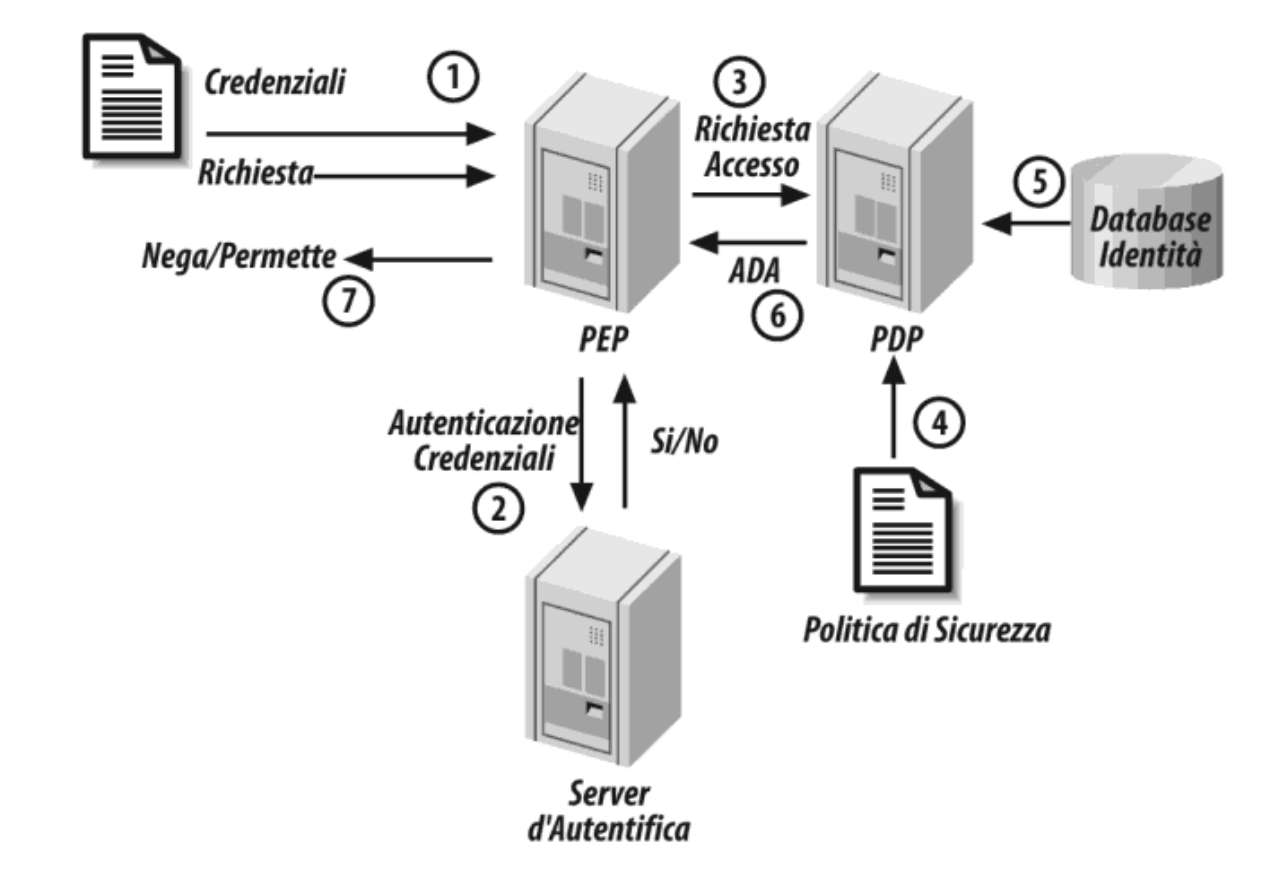
\includegraphics[width=320bp]{img/sistema_autenticazione.png}
		\caption{Sistema di autenticazione di un'identità digitale}
	\end{center}
\end{figure}

\subsection{Dati personali e privacy}
Spesso l'identità digitale coincide con i dati personali di un individuo, sopratutto quando ad erogare servizi e assegnare accessi a risorse è un ente pubblico che ha necessariamente bisogno di conoscere la persona fisica.

diritto alla riservatezza

vecchio codice privacy italiano

gdpr art.4 definizione di dato personale 

trattamento dei dati personali in UE, USA e CINA

\subsection{Tutela dei dati personali}
 gdpr diritto all'oblio
 %https://books.google.it/books?hl=it&lr=&id=45RWCwAAQBAJ&oi=fnd&pg=PA5&dq=identit%C3%A0+digitale&ots=CbIBWkFRVU&sig=XFjPDH-3_ADHim0yD5kLRFgE_JE&redir_esc=y#v=onepage&q=identit%C3%A0%20digitale&f=false
\subsection{Furto d'identità}

https://dialnet.unirioja.es/servlet/articulo?codigo=6155941

\section{Perchè profilare}


\section{Metodi di profilazione}
\subsection{Profilazione utente implicita}
\subsection{Profilazione utente esplicita}
\subsection{Profilazione ibrida}
\section{Techiche di profilazione}
\subsection{Profile extraction}
\subsection{Profile integration}
\subsection{Interest discovery}


\section{Profilazione nelle Smart City}



%TCP/IP over Avian Carriers\cite{waitzman1990standard}

